\subsection{모델 아키텍처}
\label{sec:architecture}

PRAGMA는 인코더 전용 트랜스포머로서, 이벤트 이력과 맥락 속성을 입력받아 레코드 수준의 밀집(dense) 임베딩을 출력한다.
이 모델은 마스킹된 입력 토큰을 복원하는 마스킹 모델링(masked modelling, MLM) 목적함수(objective)로, 대규모이면서 다양성이 큰 데이터셋 위에서 학습된다.
사전학습이 끝나면 백본 역할을 하며, 다양한 다운스트림 과제에 대해 모델 파라미터의 2--4\,\%만 갱신하는 소규모 파인튜닝으로 적응시킬 수 있다.
PRAGMA의 개요는 그림~\ref{fig:method}에 제시되어 있다.

\begin{figure}
    \centering
    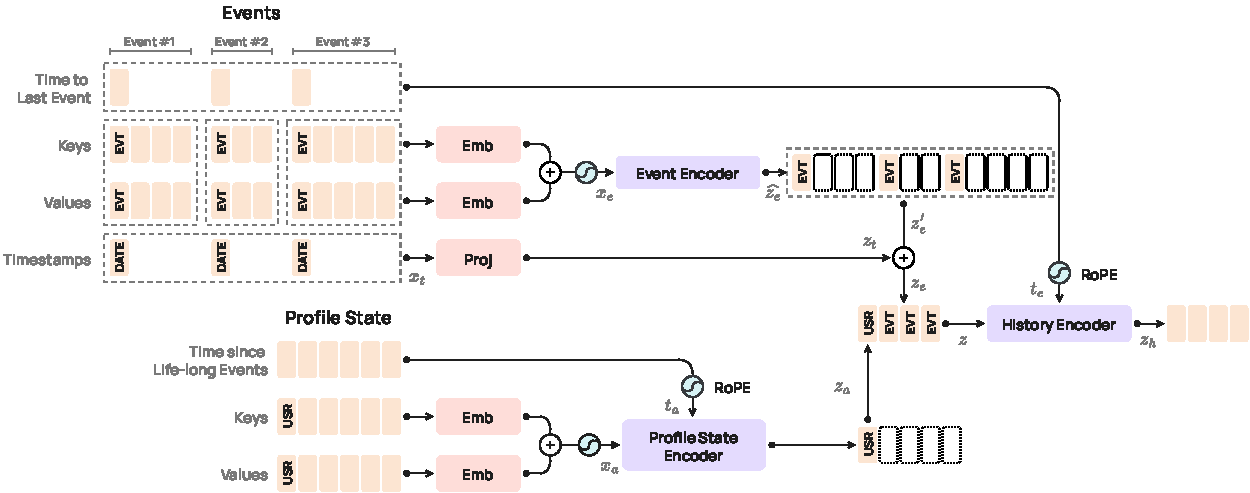
\includegraphics[width=1\linewidth]{images/method.pdf}
    \caption{
        \textbf{PRAGMA 백본 개요}.
        각 사용자 레코드는 시간순 이벤트 이력과 프로필 상태로 표현되며, 모든 필드는 의미 타입(키), 하나 이상의 값, 그리고 시간 좌표로 분해된다.
        키와 값은 공유 룩업 테이블에서 임베딩되며, 값 토큰에는 필드 내(within-field) 위치 임베딩이 더해진다.
        \emph{프로필 상태 인코더}는 프로필 상태 $x_a$를, 라이프롱 이벤트로부터의 시간 $t_a$를 RoPE로 인코딩하며 \texttt{[USR]} 임베딩 $z_a$로 매핑한다.
        한편 \emph{이벤트 인코더}는 각 이벤트의 토큰 $x_e$를 독립적으로 \texttt{[EVT]} 임베딩 $z_e'$로 매핑하고 달력 피처 $z_t$를 더한다.
        그 다음, \emph{히스토리 인코더}가 직전 이벤트까지의 시간 $t_e$를 RoPE로 인코딩하면서 시퀀스 $z=[z_a:z_e]$를 맥락화하여 사용자 레코드 표현 $z_h$를 만들어낸다.
    }
    \label{fig:method}
\end{figure}

PRAGMA는 10\,M, 100\,M, 1\,B 파라미터의 모델 계열로 파라미터화되어 있어, 운영 예산과 제약에 따라 선택할 수 있다.
아키텍처 계열의 세부 사항은 표~\ref{tab:model_family}에 제시되어 있다.
모든 사이즈 변형은 GELU 활성 함수(activation function)~\citep{hendrycks2016gaussian}, 사전 정규화(pre-norm) 레이어 정규화(layer normalisation)~\citep{xiong2020layer}, 0.1의 드롭아웃(dropout)~\citep{srivastava2014dropout}을 사용한다.

\begin{table}[t]
    \centering
    \begin{tabular}{lr rr rrr r}
        & & \multicolumn{2}{c}{\textbf{Width}} & \multicolumn{3}{c}{\textbf{Depth}} & \\
        \cmidrule(lr){3-4} \cmidrule(lr){5-7}
        \textbf{모델} & \textbf{파라미터} & \textbf{$d_{\mathrm{model}}$} & \textbf{$d_{\mathrm{ffn}}$} & \textbf{Profile} & \textbf{Event} & \textbf{History} & \textbf{Heads} \\
        \midrule
        PRAGMA-S &  10\,M & 192  & 768  & 1 & 5  & 2  & 3  \\
        PRAGMA-M & 100\,M & 512  & 2048 & 3 & 16 & 6  & 8  \\
        PRAGMA-L &   1\,B & 1024 & 4096 & 9 & 45 & 18 & 16 \\
    \end{tabular}
    \caption{
        \textbf{PRAGMA 모델 계열}.
        PRAGMA는 모델 폭($d_{\mathrm{model}}$, $d_{\mathrm{ffn}}$), 프로필 상태·이벤트·히스토리 인코더의 깊이, 그리고 어텐션 헤드 수를 함께 키우면서 10\,M, 100\,M, 1\,B 파라미터의 세 변형으로 확장된다.
    }
    \label{tab:model_family}
\end{table}

모델은 세 개의 주요 블록으로 구성된다 — 프로필 상태 인코더, 이벤트 인코더, 히스토리 인코더.
첫째, 프로필 상태 토큰은 프로필 상태 인코더가 처리한다.
둘째, 프로필 상태와 마찬가지로 각 이벤트는 이벤트 인코더에서 독립적으로 인코딩된다.
마지막으로, 프로필 상태 인코더와 이벤트 인코더의 출력을 연결한 뒤 히스토리 인코더에 통과시켜 출력을 만든다.
단계에 따라 최종 출력은 사전학습 시 MLM 헤드(head), 파인튜닝 시 분류 헤드(classification head), 또는 임베딩 프로브(embedding probe)에서 그대로 사용된다.

\subsubsection{토큰 임베딩}
\label{sec:token_embedding}
프로필 상태와 이벤트 토큰은 동일한 방식으로 임베딩된다.
다중값을 갖는 필드(예: \texttt{Description})에서는, 키 토큰이 각 값에 맞춰 복제되어 총 $n$개의 키--값 쌍이 만들어진다.
공유된 단일 임베딩 테이블 $E$가 각 키와 값을 $d$차원 벡터로 매핑하며, 두 임베딩은 합산된 뒤 정적 사인/코사인 위치 인코딩(PosEmb)~\citep{vaswani2017attention}으로 보강된다:
\begin{align}
    x = \text{PosEmb}\big(E(k) + E(v)\big), \quad x \inR^{n \times d}.
\end{align}
위치 인덱스는 필드 사이가 아니라 필드 \emph{안}에서의 값 위치를 가리킨다 — 예컨대, \texttt{Currency}의 값 \texttt{eur}은 위치 \texttt{0}을, \texttt{Description}의 세 값 토큰 \texttt{(met,\,al,\,plan)}은 위치 \texttt{(0,\,1,\,2)}를 받는다(그림~\ref{fig:tokenisation} 참조).
저자들은 사용자(프로필) 임베딩을 $x_a \inR^{n_a \times d}$, 이벤트 임베딩을 $x_e \inR^{n_e \times d}$로 표기한다.
인코더 전용 트랜스포머의 일반 관행을 따라~\citep{devlin2019bert,dosovitskiy2021image}, 학습 가능한 \texttt{[USR]}(또는 \texttt{[EVT]}) 토큰을 각 시퀀스 앞에 붙인다(그림~\ref{fig:method}).


\subsubsection{프로필 상태 인코더}
프로필 상태 인코더는 양방향 트랜스포머다.
입력은 프로필 상태 토큰 $x_a \inR^{n_a \times d}$와 이에 대응하는 시간 좌표 $t_a \inR^{n_a}$이며, 각 항목은 해당 라이프롱 이벤트로부터의 로그-초를 담는다(라이프롱이 아닌 쌍은 $0$).
$t_a$는 RoPE~\citep{su2024roformer}로 인코딩한다.
이 위치 임베딩은 \S\ref{sec:token_embedding}에서 다룬 값 수준 위치 임베딩과 분리(disentangle)해, 의미적·스케일적 불일치를 피한다.
출력은 프로필 상태 임베딩 시퀀스 $z_a\inR^{n_a \times d}$이다.
\texttt{[USR]} 토큰에 해당하는 첫 원소를 히스토리 인코더로 전달하며, 표기 단순화를 위해 이를 $z_a\inR^{1 \times d}$로 부른다.

\subsubsection{이벤트 인코더}
\label{sec:event_encoder}
이벤트 인코더는 프로필 상태 인코더와 비슷한 양방향 트랜스포머다.
입력은 이벤트 이력 $x_e = (x_{e, 1}, x_{e, 2}, \dots, x_{e, n_e})$이며, 각 원소는 서로 다른 수의 토큰 임베딩을 갖고($x_{e,i} \inR^{n_i \times d}$), 이력 안의 다른 모든 이벤트와 독립적으로 처리된다.
이 모듈은 각 이벤트에 대해 토큰 수준의 임베딩 시퀀스 $\widehat{z}_e$를 출력하며, 이 출력은 사전학습 시 MLM 헤드가 사용한다.
프로필 상태 인코더와 마찬가지로, 각 이벤트의 \texttt{[EVT]} 토큰에 해당하는 첫 토큰을 그 이벤트의 집계 표현 $z_e' \inR^{n_e \times d}$으로 선택한다.

달력 피처(시각의 시, 요일, 일자) $x_t\inR^{n_e\times 3}$는 사인·코사인 라디안으로 변환된 뒤 두 개의 MLP 층으로 임베딩되어 $z_t\inR^{n_e \times d}$가 된다.
그 다음, 이 임베딩된 달력 피처를 이벤트 인코더 출력에 더한다 — $z_e = z_e' + z_t$.

\subsubsection{히스토리 인코더}
히스토리 인코더는 다른 두 인코더와 비슷한 양방향 트랜스포머다.
입력은 프로필 상태와 달력 피처가 더해진 이벤트의 집계 표현을 이은 시퀀스 $z=[z_a:z_e] \inR^{(1+n_e) \times d}$, 그리고 대응하는 시간 좌표 $t_e \inR^{1+n_e}$이며, 각 항목은 이력 안에서 가장 최근 이벤트까지의 로그-초를 담는다($z_a$ 자리는 $0$).
프로필 상태 인코더와 마찬가지로, 위치 정보 인코딩에는 RoPE를 사용한다.
출력은 임베딩 시퀀스 $z_h\inR^{(1+n_e)\times d}$이며, $z_{h,0}$은 \texttt{[USR]}에, $z_{h,1},\dots,z_{h,n_e}$는 \texttt{[EVT]} 토큰들에 해당한다.
$z_h$는 사전학습 시 MLM 헤드, 그리고 다운스트림 프로브에 사용된다.

\subsubsection{학습}
\label{sec:training}
\paragraph*{사전학습 목적함수.}
PRAGMA는 BERT~\citep{devlin2019bert}를 따라 MLM 목적함수로 사전학습된다 — 이벤트 입력 토큰의 임의 부분집합을 마스킹하고, 모델은 원래 토큰을 복원한다.
각 마스킹된 토큰에 대해, MLM 헤드는 세 개의 $d$차원 벡터를 이어붙인 입력을 받는다 — $\widehat{z}_e$ 안에서 그 토큰 위치에 해당하는 이벤트 인코더 출력(이벤트 내 지역적 맥락), 대응되는 \texttt{[EVT]} 위치의 히스토리 인코더 출력 $z_{h,i}$(이벤트 간 맥락), 그리고 \texttt{[USR]} 위치의 히스토리 인코더 출력 $z_{h,0}$(사용자 수준 맥락).
이 $3d$차원 표현은 다시 $d$차원으로 사영된 뒤, 임베딩 테이블과의 매칭을 통해 logit으로 만들어진다.
학습 손실은 라벨 스무딩(label smoothing)이 적용된 교차 엔트로피(cross entropy)이다~\citep{szegedy2016rethinking}.

\paragraph*{마스킹 전략.}
마스킹 전략은 세 가지 경로를 결합한다 — 표준적인 토큰 단위 마스킹(15\,\% 확률), 모델이 이벤트 전체를 복원하게 하는 이벤트 단위 마스킹(10\,\%), 그리고 선택된 키의 모든 값을 마스킹하여 키와 맥락이 주어졌을 때 값을 예측하게 하는 의미 타입(키) 단위 마스킹(10\,\%).
사전학습 동안에는, 선택된 위치 중 일부를 \texttt{[MASK]} 대신 \texttt{[UNK]}로 바꾼다.
\texttt{[UNK]} 위치는 MLM 목적함수에서 제외되어 그래디언트를 받지 않으므로, 사실상 입력 드롭아웃의 한 형태로 작동한다. 이는 더 강한 변형(corruption) 아래에서도 원래 값을 복원하도록 학습시키고, 추론 시에는 등장하지 않는 \texttt{[MASK]}에 대한 의존을 줄여 준다.

\paragraph*{다운스트림 적응.}
PRAGMA는 두 가지 다운스트림 적응 모드를 지원한다.
\emph{임베딩 프로브 모드}에서는 히스토리 인코더가 만들어 낸 레코드 수준 표현을 고정된 피처 벡터로 추출한 뒤, 그 위에 가벼운 선형 프로브를 학습한다.
\emph{LoRA 파인튜닝 모드}에서는 모델 가중치(어텐션과 피드포워드 사영(projection))의 작은 일부(약 2--4\,\%)를 Low-Rank Adaptation~\citep{hu2022lora}으로 갱신한다. 이는 사전학습 백본을 거의 그대로 동결시켜 파국적 망각(catastrophic forgetting)의 위험을 줄여 준다.
